\documentclass[tikz,border=5pt]{standalone}

\usepackage{tikz}
\usetikzlibrary{arrows.meta}
\usepackage{siunitx}

\begin{document}

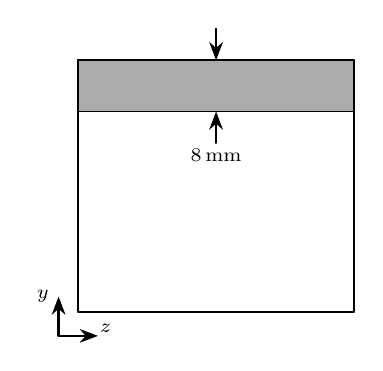
\begin{tikzpicture}[
    line cap=round,
    line join=round,
    >=Stealth
]

% Outer square
% \draw[line width=0.6pt] (0,0) rectangle (4,4);

% Inner square
\draw[line width=0.6pt] (0.25,0.4) rectangle (3.75,3.6);

% Dark grey bar
\fill[gray!65] (0.25,3.6) rectangle (3.75,2.95);
\draw[line width=0.6pt] (0.25,3.6) rectangle (3.75,2.95);

% Black lower edge of the bar
% \fill[black] (0.48,2.35) rectangle (3.52,2.29);

% Small white gaps at top of grey bar
% \draw[white,line width=1.0pt] (0.85,2.95) -- (1.15,2.95);
% \draw[white,line width=1.0pt] (2.85,2.95) -- (3.15,2.95);

% Central vertical dimension line
% \draw[thick] (2.0,3.6) -- (2.0,2.95);

% Top downward arrow
\draw[->, thick] (2.0, 4.0) -- (2.0, 3.6);

% Bottom upward arrow
\draw[<-, thick] (2.0, 2.95) -- (2.0, 2.55);

% Dimension text
\tikzset{label font/.style={font=\fontsize{7pt}{10pt}\selectfont}}

\node[label font] at (2.0,2.4)
  {\qty{8}{\milli\metre}};

% Coordinate system
    \draw[thick, ->] (0.0,0.1) -- (0.5,0.1);
    \node[label font, anchor=west] at (0.4, 0.2) {$z$};
    \draw[thick, ->] (0.0,0.1) -- (0.0,0.6);
    \node[label font, anchor=east] at (0.0, 0.6) {$y$};


\end{tikzpicture}

\end{document}